\section{Metasploit}
Metasploit è stato utilizzato come port scan nella sua versione di default e successivamente abilitando l'opzione \textit{Scan SNMP}.\\
Dai grafici si nota come la versione standard dell'attacco di Metasploit sia più corta rispetto alla versione completa, probabilmente a causa delle operazioni in più che quest'ultima compie. Inoltre possiamo vedere che il tempo di detection dell'attacco standard è più alto rispetto alla versione avanzata, che invece viene rilevata subito da Snort, forse a causa delle tecniche di intrusione più aggressive introdotte da quest'ultima.\\

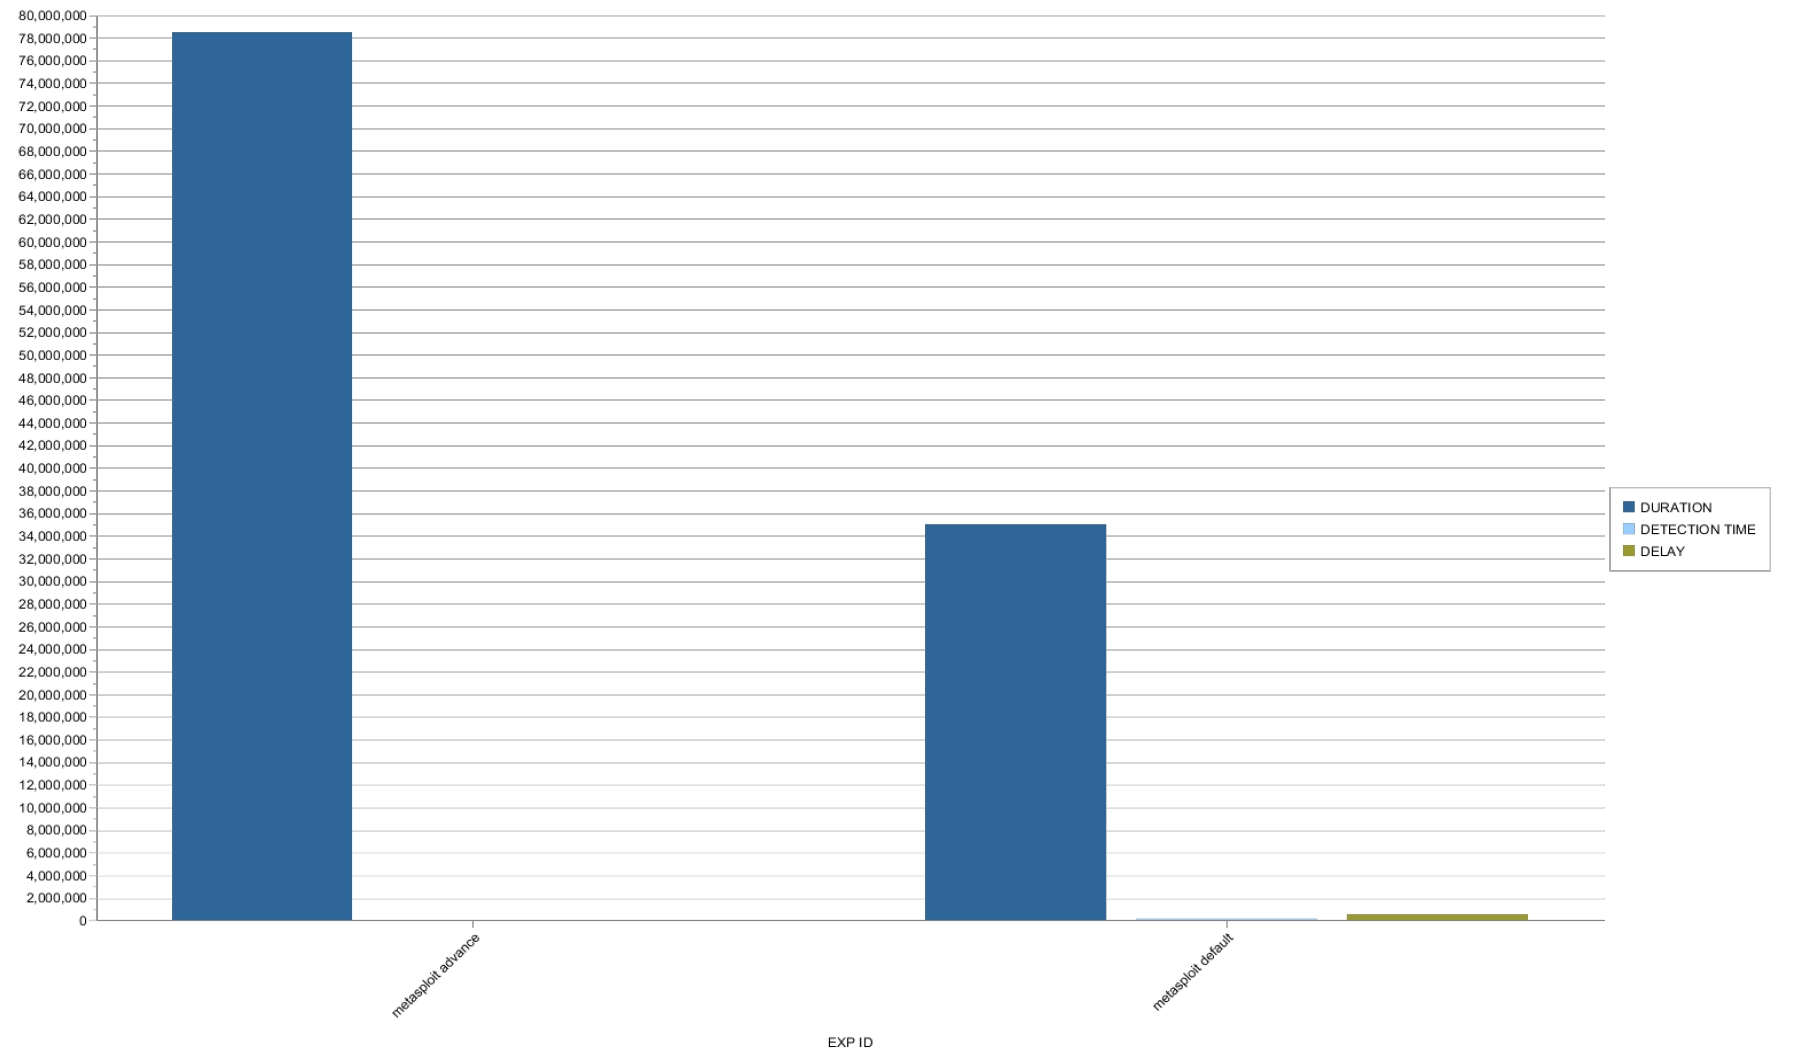
\includegraphics[scale=0.3]{figure/grafico_metasploit.jpg}\\

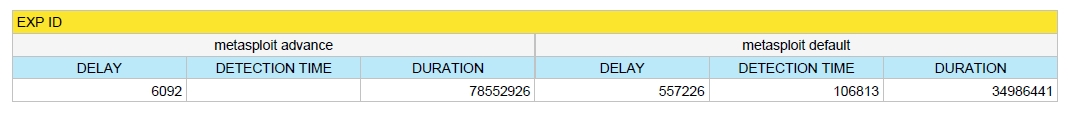
\includegraphics[scale=0.3]{figure/tempi_metasploit.jpg}

